\section{Verificações Preditivas}

\subsection{Leituras Recomendadas}
\begin{frame}{Verificações Preditivas - Leituras Recomendadas}
	\begin{vfilleditems}
		\item \textcite{gelman2013bayesian} - Capítulo 6: Model checking
		\item \textcite{mcelreath2020statistical} - Capítulo 5: Geocentric Models
		\item \textcite{gelman2020regression}:
		\begin{vfilleditems}
			\item Capítulo 6: Background on regression modeling
			\item Capítulo 11: Assumptions, diagnostics, and model evaluation
		\end{vfilleditems}
		\item \textcite{gelmanBayesianWorkflow2020}
	\end{vfilleditems}
\end{frame}

\subsection{All models are wrong}
\begin{frame}{\textit{All models are wrong}}
	\begin{columns}
		\begin{column}{0.8\textwidth}
			\begin{quotation}
				All models are wrong but some are useful
			\end{quotation}
			\vfill
			\textcite{boxScienceStatistics1976}
		\end{column}
		\begin{column}{0.2\textwidth}
			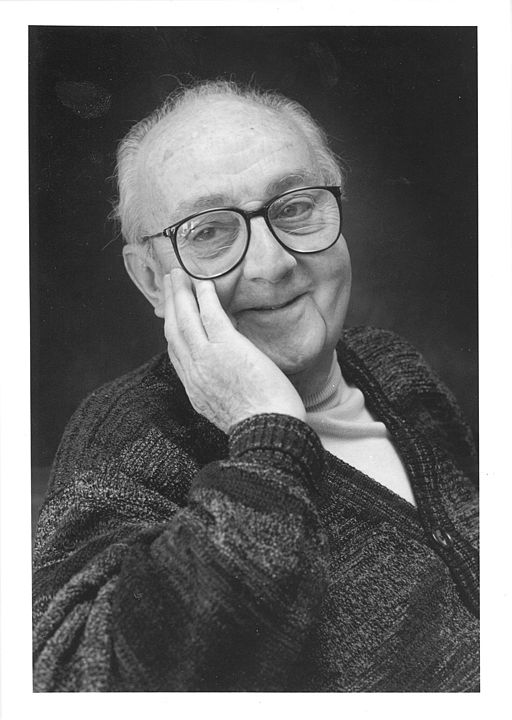
\includegraphics[width=0.9\columnwidth]{george_box.jpg}
		\end{column}
	\end{columns}
\end{frame}

\subsection{Fluxo de Trabalho Bayesiano (\textit{Workflow})\footnote{baseado em \textcite{gelmanBayesianWorkflow2020}}}
\begin{frame}{Fluxo de Trabalho Bayesiano (\textit{Workflow})\footnote{baseado em \textcite{gelmanBayesianWorkflow2020}}}
	\centering
	\begin{tikzpicture}[
			scale=0.8,
			transform shape, thick,
			every node/.style={text width=3.5cm, align=center},
			constructs/.style = {draw,
					ellipse,
					minimum width=4cm,
					minimum height=2cm}
		]
		\node[constructs] (Modelo) {Especificação do Modelo};
		\node[constructs] [right = of Modelo] (Priori) {Elicitação das \textit{Prioris}};
		\node[constructs] [right = of Priori] (Posterior) {Inferência da Posterior};
		\draw [<->, line width=1pt] (Modelo) to [out=45,in=135] node[above] {\textit{Prior Predictive Check}} (Priori);
		%\draw [->, line width=1pt] (Priori) to [out=225,in=315] {} (Modelo);
		\draw [<->, line width=1pt] (Priori) to [out=45,in=135] node[above] {\textit{Posterior Predictive Check}} (Posterior);
		%\draw [->, line width=1pt] (Posterior) to [out=225,in=315] {} (Priori);
	\end{tikzpicture}
\end{frame}

\subsection{Verificação Preditiva da \textit{Priori} (\textit{Prior Predictive Check})}
\begin{frame}{Verificação Preditiva da \textit{Priori} (\textit{Prior Predictive Check})}
	Em especial, antes de começar a alimentar o modelo com dados precisamos fazer uma
	checagem de todas as nossas \textit{prioris}.
	\vfill
	De maneira muito simples, consiste em simular parâmetros com base nas suas distribuições
	especificadas \textit{a priori} no modelo sem qualquer condicionamento aos dados e
	sem envolvimento nenhum da função de verossimilhança.
	\vfill
	Independentemente do nível de informação especificada na \textit{priori},
	é sempre importante realizar uma análise de sensibilidade prévia para entender completamente
	a influência que as \textit{prioris} têm na posterior.
\end{frame}

\begin{frame}{Verificação Preditiva da \textit{Priori} no \href{http://mc-stan.org/rstanarm/}{\texttt{rstanarm}} e \href{https://paul-buerkner.github.io/brms/}{\texttt{brms}}}
	\begin{vfilleditems}
		\item \texttt{rstanarm}: em qualquer função \text6t{stan\_*()} usar o argumento \texttt{prior\_PD = TRUE}
		\item \texttt{brms}: na função \textit{brm()} usar o argumento \texttt{sample\_prior = "only"}
	\end{vfilleditems}
\end{frame}

\subsubsection{Verificação Preditiva da \textit{Priori} no \texttt{rstanarm}}
\begin{frame}[fragile]{Verificação Preditiva da \textit{Priori} no \href{http://mc-stan.org/rstanarm/}{\texttt{rstanarm}}}
	\begin{lstlisting}
    stan_glm(y ~ ...,
        prior = normal(c(0, 0), c(5, 6)),
        prior_intercept = student_t(4, 0, 10),
        prior_aux = cauchy(0, 3),
        @prior_PD = TRUE@)
    \end{lstlisting}
\end{frame}
\subsubsection{Verificação Preditiva da \textit{Priori} no \texttt{brms}}
\begin{frame}[fragile]{Verificação Preditiva da \textit{Priori} no \href{https://paul-buerkner.github.io/brms/}{\texttt{brms}}}
	\begin{lstlisting}
    brm(y ~ x1 + x2,
        prior = c(
          prior(normal(0, 5), class = b, coef = x1),
          prior(normal(0, 6), class = b, coef = x2),
          prior(student_t(4, 0, 10), class = Intercept),
          prior(cauchy(0, 3), class = sigma)
        ),
        @sample_prior = "only"@)
    \end{lstlisting}
\end{frame}

\begin{frame}{Verificação Preditiva da \textit{Priori} no \href{https://paul-buerkner.github.io/brms/}{\texttt{brms}}}
	O interessante do \href{https://paul-buerkner.github.io/brms/}{\texttt{brms}} é
	que conseguimos naturalmente visualizar hipóteses sobre os valores do parâmetros de modelos
	estimados pela função \lstinline!brm()!
	% library(brms)
	% library(ggplot2)
	% library(ggdark)
	% library(bayesplot)
	% library(tikzDevice)
	% theme_set(dark_theme_light())
	% bayesplot_theme_set(dark_theme_light())
	% brms_custom_prior <- brm(mpg ~ wt + am, data = mtcars, chains = 1,
	%  prior = c(
	%    prior(normal(0, 5), class = b, coef = wt),
	%    prior(normal(0, 6), class = b, coef = am),
	%    prior(student_t(4, 0, 10), class = Intercept),
	%    prior(cauchy(0, 3), class = sigma)
	%  ),
	%  sample_prior = "only")
	% tikz(file = "slides/images/brms_prior_check.tex")
	% plot(hypothesis(brms_custom_prior, "Intercept = 0"))
	% dev.off()
	\begin{figure}
		\centering
		\resizebox{.35\linewidth}{!}{\input{images/brms_prior_check.tex}}
	\end{figure}
\end{frame}

\subsection{Verificação Preditiva da Posterior (\textit{Posterior Predictive Check})}
\begin{frame}{Verificação Preditiva da Posterior (\textit{Posterior Predictive Check})}
	Precisamos nos certificar que a nossa distribuição posterior de $\boldsymbol{y}$
	consegue capturar todas as nuanças da densidade real de $\boldsymbol{y}$.
	\vfill
	Isto é um procedimento chamado de Verificação Preditiva da Posterior
	(\textit{Posterior Predictive Check}) e é geralmente auferido com uma inspeção
	visual\footnote{também fazemos inspeções matemáticas probabilísticas,
		veja a seção de Comparação de Modelos} da densidade real de $\boldsymbol{y}$
	contrastada com amostragens da densidade
	posterior de $\boldsymbol{y}$ estimada pelo modelo Bayesiano.
	\vfill
	O propósito é comparar o histograma da variável dependente $\boldsymbol{y}$ contra o histograma variáveis dependentes simuladas
	pelo modelo $\boldsymbol{y}_{\text{rep}}$ após a estimação dos parâmetros. A ideia é
	que os histogramas reais e simulados se misturem e não haja divergências.
\end{frame}

\begin{frame}{Verificação Preditiva da Posterior no \href{http://mc-stan.org/rstanarm/}{\texttt{rstanarm}} e \href{https://paul-buerkner.github.io/brms/}{\texttt{brms}}}
	\begin{vfilleditems}
		\item \texttt{rstanarm}: função \lstinline!pp_check()! em qualquer modelo oriundo das funções \lstinline!stan_*()!
		\item \texttt{brms}: função \lstinline!pp_check()! em qualquer modelo oriundo da função \lstinline!brm()!
	\end{vfilleditems}
\end{frame}

\subsubsection{Verificação Preditiva da Posterior no \texttt{rstanarm}}
\begin{frame}[fragile]{Verificação Preditiva da Posterior no \href{http://mc-stan.org/rstanarm/}{\texttt{rstanarm}}}
	\begin{lstlisting}
    rstanarm_fit <- stan_glm(mpg ~ wt + am, data = mtcars)
    @pp_check(rstanarm_fit)@
    \end{lstlisting}
\end{frame}

\begin{frame}{Verificação Preditiva da Posterior no \href{http://mc-stan.org/rstanarm/}{\texttt{rstanarm}}}
	% library(rstanarm)
	% library(ggplot2)
	% library(ggdark)
	% library(bayesplot)
	% library(tikzDevice)
	% theme_set(dark_theme_light())
	% bayesplot_theme_set(dark_theme_light())
	% rstanarm_fit <- stan_glm(mpg ~ wt + am, data = mtcars)
	% tikz(file = "slides/images/pp_check_rstanarm.tex")
	% pp_check(rstanarm_fit, nreps = 10, seed = 123, type = "dens_overlay")
	% dev.off()
	\begin{columns}
		\begin{column}{0.5\textwidth}
			\begin{figure}
				\centering
				\resizebox{0.8\columnwidth}{!}{\input{images/pp_check_rstanarm.tex}}
			\end{figure}
		\end{column}
	\end{columns}
\end{frame}

\subsubsection{Verificação Preditiva da Posterior no \texttt{brms}}
\begin{frame}[fragile]{Verificação Preditiva da Posterior no \href{https://paul-buerkner.github.io/brms/}{\texttt{brms}}}
	O interessante do \href{https://paul-buerkner.github.io/brms/}{\texttt{brms}} é
	que conseguimos olhar o PPC da distribuição CDF empírica (\textit{ECDF}) também:
	\vfill
	\begin{lstlisting}
    brms_fit <- brm(mpg ~ wt + am, data = mtcars)
    @pp_check(brmsfit)@
    @pp_check(brmsfit, type = "ecdf_overlay")@
    \end{lstlisting}
\end{frame}

\begin{frame}{Verificação Preditiva da Posterior no \href{https://paul-buerkner.github.io/brms/}{\texttt{brms}}}
	% library(brms)
	% library(ggplot2)
	% library(ggdark)
	% library(bayesplot)
	% library(tikzDevice)
	% theme_set(dark_theme_light())
	% bayesplot_theme_set(dark_theme_light())
	% brms_fit <- brm(mpg ~ wt + am, data = mtcars)
	% tikz(file = "slides/images/pp_check_brms.tex")
	% pp_check(brms_fit, nreps = 10, seed = 123)
	% dev.off()
	% tikz(file = "slides/images/pp_check_brms_ecdf.tex")
	% pp_check(brms_fit, nreps = 10, seed = 123, type = "ecdf_overlay")
	% dev.off()
	\begin{columns}
		\begin{column}{0.5\textwidth}
			\begin{figure}
				\centering
				\resizebox{0.8\columnwidth}{!}{\input{images/pp_check_brms.tex}}
			\end{figure}
		\end{column}
		\begin{column}{0.5\textwidth}
			\begin{figure}
				\centering
				\resizebox{0.8\columnwidth}{!}{\input{images/pp_check_brms_ecdf.tex}}
			\end{figure}
		\end{column}
	\end{columns}
\end{frame}
